\documentclass{article}

%% Page Margins %%
\usepackage{geometry}
\geometry{
    top = 0.75in,
    bottom = 0.75in,
    right = 0.75in,
    left = 0.75in,
}

\usepackage{amsmath}
\usepackage{graphicx}
\usepackage{parskip}

\title{Assembly Project: Dr Mario}

% TODO: Enter your name
\author{Roy Liu}

\begin{document}
\maketitle

\section{Instruction and Summary}

\begin{enumerate}

    \item Which milestones were implemented? 
    % TODO: List the milestone(s) and in the case of 
    %       Milestones 4 & 5, list what features you 
    %       implemented, sorted into easy and hard 
    %       categories.
    
    Milestone 1
    
    Milestone 2
    
    Milestone 3
    
    Milestone 4 \& 5
    \begin{itemize}

    \item 1. Gravity
    \item 2. Increase Gravity Overtime
    \item 3. Difficulty Selection
    \item 4. Retry Screen
    \item 6. Pause Message
    \item 11. Next Capsule
    \item 12. Next 4 Capsules
    \item 15. Save Capsule
    
    \end{itemize}

    \item How to view the game:
    % TODO: specify the pixes/unit, width and height of 
    %       your game, etc.  NOTE: list these details in
    %       the header of your breakout.asm file too!
    
    \begin{enumerate}
    
    \item Unit width in pixels:       1
    \item Unit height in pixels:      1
    \item Display width in pixels:    32
    \item Display height in pixels:   32
    \item Base Address for Display:   0x10008000 (\$gp)


    \end{enumerate}

    

\begin{figure}[ht!]
    \centering
    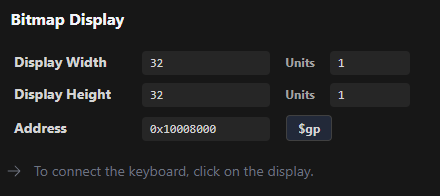
\includegraphics[width=0.3\textwidth]{bitmap_config.png}
    \caption{Bitmap configuration in Saturn}
    \label{Instructions}
\end{figure}

\item Game Summary:
% TODO: Tell us a little about your game.
\begin{itemize}
\item At anytime, you can press 'q' to quit the game.
\item The main menu has 3 options: easy, medium, and hard. You can select them by hitting the corresponding key shown on screen.
\item Viruses are lighter shades of the capsule colours in the bottle.
\item Viruses are cleared when matched in a line of the same colour that's 4 or more longer, like the original Dr. Mario.
\item The game automatically ends when all viruses are cleared.
\item If the top of the bottle is blocked, a game over shows, and you can press 'r' to retry the game.

Controls: 

\item W: rotate clockwise
\item A: move left
\item S: move down
\item D: move right
\item C: save capsule / switch with saved capsule
\item P: pause game
\end{itemize}

    
\end{enumerate}

\section{Attribution Table}
% TODO: If you worked in partners, tell us who was 
%       responsible for which features. Some reweighting 
%       might be possible in cases where one group member
%       deserves extra credit for the work they put in.

\begin{center}
\begin{tabular}{|| c | c ||}
\hline
 Student 1 (Roy Liu, 1010331062) \\ 
 \hline
 EVERYTHING\\
 \hline
\end{tabular}
\end{center}

% TODO: Fill out the remainder of the document as you see 
%       fit, including as much detail as you think 
%       necessary to better understand your code. 
%       You can add extra sections and subsections to 
%       help us understand why you deserve marks for 
%       features that were more challenging than they
%       might initially seem.
\section{Milestone Figures}

\begin{figure}[ht!]
    \centering
    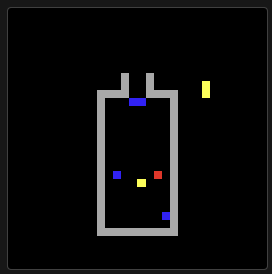
\includegraphics[width=0.3\textwidth]{milestone_1.png}
    \caption{Milestone 1 Bitmap}
    \label{Instructions}
\end{figure}

\begin{figure}[ht!]
    \centering
    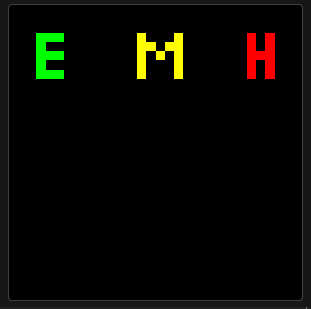
\includegraphics[width=0.3\textwidth]{main_menu.png}
    \caption{Main Menu}
    \label{Instructions}
\end{figure}

\begin{figure}[ht!]
    \centering
    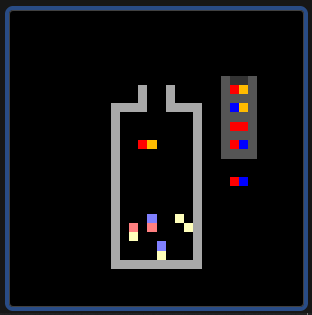
\includegraphics[width=0.3\textwidth]{gameplay.png}
    \caption{Gameplay}
    \label{Instructions}
\end{figure}

\begin{figure}[ht!]
    \centering
    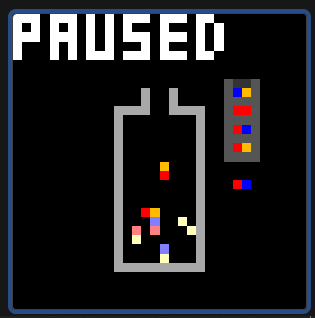
\includegraphics[width=0.3\textwidth]{paused_message.png}
    \caption{Paused Message}
    \label{Instructions}
\end{figure}

\begin{figure}[ht!]
    \centering
    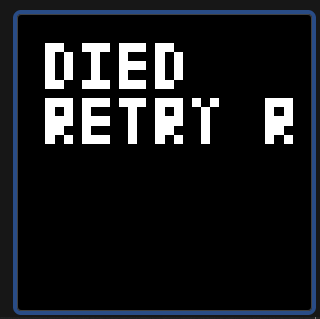
\includegraphics[width=0.3\textwidth]{retry_screen.png}
    \caption{Game Over Screen}
    \label{Instructions}
\end{figure}

\begin{figure}[ht!]
    \centering
    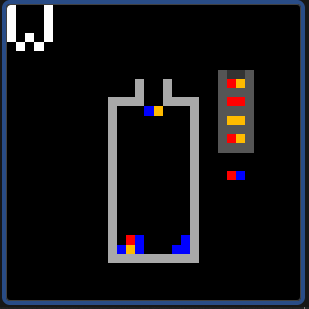
\includegraphics[width=0.3\textwidth]{win_screen.png}
    \caption{Win Message}
    \label{Instructions}
\end{figure}

\end{document}